\documentclass[11pt,article]{article}
\usepackage[utf8]{inputenc}
\usepackage[T1]{fontenc} % caractères accentués en entrée, dans emacs
\usepackage[french]{babel}
\FrenchFootnotes
\selectlanguage{french}
\usepackage{a4wide} % possibilité d'utiliser toute la page a4
% selon GUT#33, avril 2007, page 13, empagement
% largeur des textes (ou justification) = 15cm
% hauteur du rectangle d'empagement = 23cm
% blanc de couture = 2/5 (21-15) = 2.4 = inner = right
% blanc de grand fond = 3/5 (21-15) = outer = left
% blanc de tête = 2/5 (29,7-23) = top
% blanc de pied = 3/5 (29,7-23) = bottom
%\usepackage[a4paper,twoside=true,right=2.4cm,left=3.6cm,top=2.68cm,bottom=4.02cm]{geometry}
% selon CFSE 2006
% - largeur des textes (ou justification) : 16cm (2cm de marge, et 1cm
%   de reliure) ;
% - hauteur des textes, y compris les notes : 23cm (2,5cm de marge
%   haute et 2cm de marge basse) ; 1ère page de : 36pts
%   d'espacement avant le titre ;
\oddsidemargin   -4mm           % 3cm a gauche des impaires
\evensidemargin   4mm           % 2cm a gauche des paires
\topmargin       -18mm          % 2.5cm en haut
\headheight       13mm          % taille de l'entete (lignes)
\headsep          24pt          % espace entre entete et texte
\footskip         30pt          % espace entre pied de page et texte
\textheight      230mm          % longeur du texte
\textwidth       160mm          % largeur du texte
\parskip 1pt                    % pas de sauts entre paragraphes
%\parindent 0pt                  % largeur de l'indentation
\usepackage{graphicx} % figure postcript avec latex,
		      % figure png avec pdflatex, au lieu d'utiliser epsfig
\usepackage[usenames,dvipsnames,table]{xcolor}
\usepackage[export]{adjustbox}
\usepackage{paralist}
\usepackage{ifthen}
\usepackage{amssymb}
\usepackage{amsfonts}
\usepackage{amsmath}
\usepackage{eurosym}
\usepackage{textcomp}
\usepackage{listings}
\lstset{language=Java,numbers=left,numberstyle=\tiny,stepnumber=4,numbersep=5pt,xleftmargin=5pt}

\usepackage{alltt}
\usepackage{longtable}

% adjust word spacing less strictly
% as result, some spaces between words may be a bit too large,
% but long words will be placed properly.
\sloppy

\newcommand{\cmt}[1]{\texttt{<}\textbf{--~#1~--}\texttt{>}}

\usepackage{lineno}
\usepackage{xspace}

\setlength{\marginparwidth}{1cm}
\setlength{\marginparsep}{10pt}
\reversemarginpar
\newcounter{usecasehaute}
\newcommand{\haute}{Haute}
\newcommand{\moyenne}{Moyenne}
\newcommand{\basse}{basse}
\newcommand{\usecase}[4]{\item \marginpar{\vspace{5pt}\ifthenelse{\equal{#1}{Haute}}{\centering\textsc{#1}\stepcounter{usecasehaute}\newline n$^{\circ}$ \theusecasehaute}{\ifthenelse{\equal{#1}{Moyenne}}{#1}{\small #1}}} #2 \begin{itemize}\item précondition~: #3 \item postcondition~: #4\end{itemize}}
\newcommand{\priorityusecase}[2]{\item \marginpar{\vspace{5pt}\ifthenelse{\equal{#1}{Haute}}{\centering\textsc{#1}\stepcounter{usecasehaute}\newline n$^{\circ}$ \theusecasehaute}{\ifthenelse{\equal{#1}{Moyenne}}{#1}{\small #1}}} #2}
\newcommand{\casusecase}[4]{\usecase{#1}{#2}{#3}{#4}}

\newcommand{\nullvalue}{\textsf{null}\xspace}
\newcommand{\emptyvalue}{\ensuremath\mathrm{vide}}
\newcommand{\invariant}{\ensuremath\mathrm{invariant}}

\begin{document}
\title{Projet CSC4102: Gestion des clefs dans un hôtel}
\author{Huang ShiHui et Mabileau Paul}
\date{Année 2019--2020~---~\today}
\maketitle

\newpage

\tableofcontents

\newpage

\section{Spécification}

\subsection{Diagrammes de cas d'utilisation}

\begin{figure}[h!]
  \includegraphics[width=1.3\textwidth,center]{DiagrammesDeCasDUtilisation/gestionclefshotel_uml_diag_cas_utilisation}
  \caption{Diagramme de cas d'utilisation du sprint 1 }
  \label{umlet_diag_cas_utilisation_du_sprint_1}
\end{figure}


\begin{figure}[h!]
  \includegraphics[width=1.3\textwidth,center]{DiagrammesDeCasDUtilisation/gestionclefshotel_uml_diag_cas_utilisation_sprint2}
  \caption{Diagramme de cas d'utilisation du sprint 2}
  \label{umlet_diag_cas_utilisation_du_sprint_2}
\end{figure}

\newpage

\subsection{Priorités, préconditions et postconditions des cas d'utilisation}

\begin{compactitem}
\subsubsection{Sprint 1}
\usecase{\haute}{Créer une chambre}
        %% précondition
        {
		\\ $\land$ identifiant de la chambre bien formé (non \nullvalue et non
          vide))
          \\ $\land$ identifiant de la chambre inexistante
		  \\$\land$ graine pour la génération des clefs bien formée (non
          \nullvalue et non vide)}
        %% postcondition
        {chambre avec ce identifiant existante}

\smallskip

\usecase{\haute}{Créer un badge d'access}
        %% précondition
         {
		  \\$\land$ identifiant de le badge bien formé (non \nullvalue et non vide)
           \\$\land$ identifiant de le badge inexistante
 		 }
        %% postcondition
         {\\chambre avec cet identifiant existante}

\smallskip

\usecase{\haute}{Créer un client}
               %% précondition
                    {
					\\$\land$ nom prénom et identifiant du client bien formées (non \nullvalue et non vide)\\
                    $\land$ client non existant dans le système}
                %% postcondition
                    {\\client enregistré dans le système}


\smallskip

            \usecase{\haute}{Enregistrer l'occupation d'une chambre par un client}
                %% précondition
                    {\\ $\land$ client existante
						$\land$ chambre existante
						$\land$ le badge d'accèss existante
                        $\land$ client occupe aucune chambre\\
                        $\land$ chambre non occupée\\
						$\land$ badge d'accèss disponible(badge n'associe aucun d'autre clients et chambres, paireClefs sont null)
						$\land$ Dernière paire de clefs de la chambre bien formé (non \nullvalue et non vide)}
                %% postcondition
                    {\\
                        $\land$ paire de clés du badge d'accès bien formées (non \nullvalue et non vide)\\
						$\land$ badge associe avec client et chambre \\
                    	$\land$ chambre occupée
						}

\smallskip

           \usecase{\haute}{Libérer une chambre}
                %% précondition
                    {\\
                        $\land$ client existante\\
						$\land$ badge existante\\
						$\land$ chambre existante\\
						$\land$ client occupe une chambre\\
						$\land$ client occupe la bonne chambre\\
                        $\land$ chambre occupée}
                %% postcondition
                    {\\
						$\land$ vider le clef du badge\\
						$\land$ disassocie les relation entre le badge et la chambre, le badge et le client \\
                    	$\land$ chambre non occupée}

\smallskip

\smallskip
\usecase{\haute}{(Re)Initialiser la serrure d'une chambre }
                %% précondition
                    {
					\\$\land$ identifiant de la serrure bien formé (non \nullvalue et non vide)\\
                    $\land$ graine et sel pour la génération des clefs bien formée (non \nullvalue et non vide)}
                %% postcondition
                    {\\serrure initialisé}

\priorityusecase{\basse}{Retirer une chambre}

\smallskip

\priorityusecase{\moyenne}{Lister les chambres}


            \subsubsection{Sprint 2}

                \usecase{\haute}{Déclarer la perte d'un badge sans remplacement}
                %% précondition
                    {\\
					badge avec ce identifiant existant\\
				}
                %% postcondition
                    {\\
					(Si le badge était en cours d'utilisation) chambre occupée par le client possédant le badge est libérée\\
					$\land$ (Si le badge était en cours d'utilisation) badge d'accès retiré du client\\
					$\land$ badge avec ce identifiant inexistant\\}

\smallskip

				\usecase{\haute}{Déclarer la perte d'un badge avec remplacement}
				%% précondition
					{\\
					badge avec ce identifiant existant
					}
				%% postcondition
					{\\

						(Si le badge était en cours d'utilisation) chambre occupée par le client possédant le badge est libérée\\
						$\land$ (Si le badge était en cours d'utilisation) badge d'accès retiré du client\\
						$\land$ badge avec ce identifiant inexistant\\
						$\land$ enregistrerOccupationChambre avec la meme client, meme chambre et d'autre badges}

                \smallskip

                \priorityusecase{\moyenne}{Notifier les doublons dans les paires de clefs et les clefs}

\end{compactitem}

\newpage

\section{Préparation des tests de validation}

\subsection{Tables de décision des tests de validation}

La fiche programme du module CSC4102 ne permettant pas de développer
des tests de validation couvrant l'ensemble des cas d'utilisation de
l'application, les cas d'utilisation choisis sont de priorité
\textsc{Haute}.

\subsubsection{Sprint 1}

\begin{table}[htbp!]
\begin{tabular}{|p{0.6\linewidth}|c|c|c|c|}
\hline
Numéro de test
&1&2&3\\
\hline

\hline
Graine pour la génération des clefs bien formée ($\neq$ \nullvalue $\land$ $\neq$ vide)
&F&T&T\\
\hline
Chambre inexistante avec ce code
& &F&T\\
\hline
\hline
Création acceptée
&F&F&T\\
\hline
\hline
Nombre de jeux de test
&2&1&1\\
\hline
\end{tabular}
\caption{Cas d'utilisation <<~créer une chambre~>>}
\end{table}
        \begin{table}[htbp!]
            \begin{tabular}{|p{0.6\linewidth}|c|c|c|c|c|c|c|c|}
                \hline
                Numéro de test
                    &1&2&3&4&5&6&7&8\\

                \hline
                Chambre existante
                    &F&T&T& & & & &T\\
                \hline
                Badge existant
                    & &F&T& & & & &T\\
				\hline
                Client existant
                    & & &F& & & & &T\\
                \hline
                \hline
                Chambre non occupée
                    & & & &F&T&T&T&T\\
                \hline
				\hline
				Client occupe aucune chambre
					& & & & &F&T&T&T\\
				\hline
				\hline
				Badge disponible
					& & & & & &F&T&T\\
				\hline
				\hline
                Dernière paire de clefs de la chambre bien formé ($\neq$ \nullvalue $\land$ $\neq$ vide)
                    & & & & & & &F&T\\
                \hline
                \hline
                Enregistrement accepté
                    &F&F&F&F&F&F&F&T\\
                \hline
                \hline
                Nombre de jeux de test
                                    &1&1&1&1&1&1&2&1\\
                \hline
            \end{tabular}
            \caption{Cas d'utilisation <<~enregistrer l'occupation d'une chambre par un client~>>}
        \end{table}

        \begin{table}[htbp!]
            \begin{tabular}{|p{0.6\linewidth}|c|c|c|c|c|c|c|c|}
                \hline
                Numéro de test
                    &1&2&3&4&5&6&7\\
                \hline
                \hline

                Chambre existante
                    &F&T&T& & & &T\\
                \hline
                Badge existant
                    & &F&T& & & &T\\
                \hline
                Client existant
                    & & &F& & & &T\\
                \hline
				\hline
                Client occupe une chambre
                    & & & &F&T&T&T\\
                \hline
                Client occupe la bonne chambre
                    & & & & &F&T&T\\
				\hline
				\hline
				Chambre occupeé
					& & & & & &F&T\\
                \hline
                \hline                Libération acceptée
                    &F&F&F&F&F&F&T\\
                \hline
                \hline
                Nombre de jeux de test
                    &1&1&1&1&1&1&2 \\
                \hline
            \end{tabular}
            \caption{Cas d'utilisation <<~libérer une chambre~>>}
        \end{table}

		\newpage

		        \subsubsection{Sprint 2}

		            \begin{table}[htbp!]
		                \begin{tabular}{|p{0.6\linewidth}|c|c|c|}
		                    \hline
		                    Numéro de test
		                        &1&2\\
		                    \hline
		                    \hline
		                   Badge avec ce identifiant existant
		                        &F&T\\
		                    \hline
		                    \hline
		                    Badge déclaré perdu acceptée
		                        &F&T\\
		                    \hline
		                    \hline
		                    Nombre de jeux de test
		                        &1&1\\
		                    \hline
		                \end{tabular}
		                \caption{Cas d'utilisation <<~déclarer la perte d'un badge d'accès~>>}
		            \end{table}
\newpage

\section{Conception}

\subsection{Liste des classes}

À la suite d'un parcours des diagrammes de cas d'utilisation et d'une
relecture de l'étude de cas, voici la liste de classes avec quelques
attributs:
\begin{compactitem}
\item \textsf{GestionClefsHotel} (la façade)
\item \textsf{Chambre}~---~identifiant, graine, sel
\item \textsf{Client}~---~identifiant, nom, prénom (ces deux derniers
  sont ajoutés ici mais ne sont pas essentiels au fonctionnement du
  système \textsf{GestionClefsHotel})
\item \textsf{Badge}~---~identifiant
\item \textsf{Clef}~---~clef
\item \textsf{PaireClefs}~---~clef1, clef2
\item \textsf{Util} (classe utilitaire déjà programmée)~---~'attribut
  de classe \textsf{TAILLE\_CLEF}, méthodes de classe
  \textsf{genererUneNouvelleClef} et \textsf{clefToString})
\end{compactitem}
\newpage

\subsection{Diagramme de classes}

\begin{figure}[h!]
  \includegraphics[width=1.3\textwidth,center]{DiagrammesDeClasses/gestionclefshotel_uml_diag_classes}
  \caption{Diagramme de classes}
  \label{umlet_diag_classes}
\end{figure}

\newpage

\subsection{Diagrammes de séquence}

\begin{figure}[h!]
  \includegraphics[width=1.3\textwidth,center]{DiagrammesDeSequence/DSUC1}
  \caption{Diagramme de séquence DSUC1 : <<Créer une chambre>>}
  \label{umlet_diag_seq1}
\end{figure}

\newpage

\begin{figure}[h!]
  \includegraphics[width=1.3\textwidth,center]{DiagrammesDeSequence/DSUC2}
  \caption{Diagramme de séquence DSUC2 : <<Enregistrer l'occupation d'une chambre par un client>>}
  \label{umlet_diag_seq2}
\end{figure}

\newpage

\begin{figure}[h!]
  \includegraphics[width=1.3\textwidth,center]{DiagrammesDeSequence/DSUC3}
  \caption{Diagramme de séquence DSUC3 : <<Libérer une chambre>>}
  \label{umlet_diag_seq3}
\end{figure}

\newpage

\begin{figure}[h!]
  \includegraphics[width=1.3\textwidth,center]{DiagrammesDeSequence/DSUC4}
  \caption{Diagramme de séquence DSUC4 : <<Déclarer le perte du badge>>}
  \label{umlet_diag_seq4}
\end{figure}
\newpage

\section{Fiche des classes}

  \subsection{Classe \textsf{GestionClefsHotel}}
  \begin{center}
	  \begin{longtable}{|p{15cm}|}
		  \hline
		  \multicolumn{1}{|c|}{{\Large \textsf{GestionClefsHotel}}} \\
		  \hline
		  \cmt{attributs <<~association~>>}\\
		  $-$ chambres: [Chambre] \\
		  $-$ badges: [Badge] \\
		  $-$ clients: [Client] \\
		  \hline
		  \cmt{constructeur} \\
		  $+$ GestionClefsHotel() \\
		  $+$ boolean invariant() \\
		  \cmt{operations <<~cas d'utilisation~>>} \\
		  $+$ Chambre creerChambre(long id, String graine, int sel) \\
		  $+$ Badge creerBadge(long id) \\
		  $+$ Client creerClient(long id, String nom, String prenom) \\
		  $+$ void enregistrerOccupationChambre(long idChambre, long idBadge, long idClient) \\
		  $+$ [Chambre] listerChambres() \\
		  $+$ void libererChambre(long id) \\
		  \cmt{opérations de recherche} \\
		  $+$ Badge chercherBadge(long id) \\
		  $+$ Chambre chercherChambre(long id) \\
		  $+$ Client chercherClient(long id) \\
		  \hline
	  \end{longtable}
  \end{center}

  \subsection{Classe \textsf{Chambre}}
  \begin{center}
	  \begin{longtable}{|p{15cm}|}
		  \hline
		  \multicolumn{1}{|c|}{{\Large \textsf{Chambre}}} \\
		  \hline
		  \cmt{attributs}\\
		  $-$ id: long \\
		  $-$ graine: String \\
		  $-$ sel: int \\
		  $-$ occupee: boolean \\
		  \cmt{attributs <<~association~>>}\\
		  $-$ paireClefs: PaireClefs \\
		  $-$ badge: Badge \\
		  \hline
		  \cmt{constructeur} \\
		  $+$ Chambre(long id, String graine, int sel) \\
		  $+$ boolean invariant() \\
		  \cmt{operations <<~cas d'utilisation~>>} \\
		  $+$ void inscrireClefs(PaireClefs paireClefs) \\
		  $+$ void liberer() \\
		  $+$ void enregistrerChambre() \\
		  \hline
	  \end{longtable}
  \end{center}

  \subsection{Classe \textsf{Badge}}
  \begin{center}
	  \begin{longtable}{|p{15cm}|}
		  \hline
		  \multicolumn{1}{|c|}{{\Large \textsf{Badge}}} \\
		  \hline
		  \cmt{attributs}\\
		  $-$ id: long \\
		  \cmt{attributs <<~association~>>}\\
		  $-$ paireClefs: PaireClefs \\
		  $-$ chambre: Chambre \\
		  $-$ client: Client \\
		  \hline
		  \cmt{constructeur} \\
		  $+$ Badge(long id) \\
		  $+$ boolean invariant() \\
		  \cmt{operations <<~cas d'utilisation~>>} \\
		  $+$ void inscrireClefs(PaireClefs paireClefs) \\
		  $+$ void vider() \\
		  $+$ void associerClient(Client client) \\
		  $+$ void associerChambre(Chambre chambre) \\
		  $+$ void dissocierClient() \\
		  \hline
	  \end{longtable}
  \end{center}

  \subsection{Classe \textsf{Client}}
  \begin{center}
	  \begin{longtable}{|p{15cm}|}
		  \hline
		  \multicolumn{1}{|c|}{{\Large \textsf{Client}}} \\
		  \hline
		  \cmt{attributs}\\
		  $-$ id: long \\
		  $-$ nom: String \\
		  $-$ prenom: String \\
		  \cmt{attributs <<~association~>>}\\
		  $-$ badge: Badge \\
		  \hline
		  \cmt{constructeur} \\
		  $+$ Client(long id, String nom, String prenom) \\
		  $+$ boolean invariant() \\
		  \hline
	  \end{longtable}
  \end{center}

  \subsection{Classe \textsf{PaireClefs}}
  \begin{center}
	  \begin{longtable}{|p{15cm}|}
		  \hline
		  \multicolumn{1}{|c|}{{\Large \textsf{PaireClefs}}} \\
		  \hline
		  \cmt{attributs}\\
		  $\#$ clef1: Clef \\
		  $\#$ clef2: Clef \\
		  \hline
		  \cmt{constructeurs} \\
          $+$ PaireClefs(Clef clef1, Clef clef2) \\
		  $+$ PaireClefs(byte[] clef1, byte[] clef2) \\
          $+$ PaireClefs() \\
		  $+$ boolean invariant() \\
		  \hline
	  \end{longtable}
  \end{center}

%\newpage

\section{Diagrammes de machine à états et invariants}


\begin{figure}[h!]
  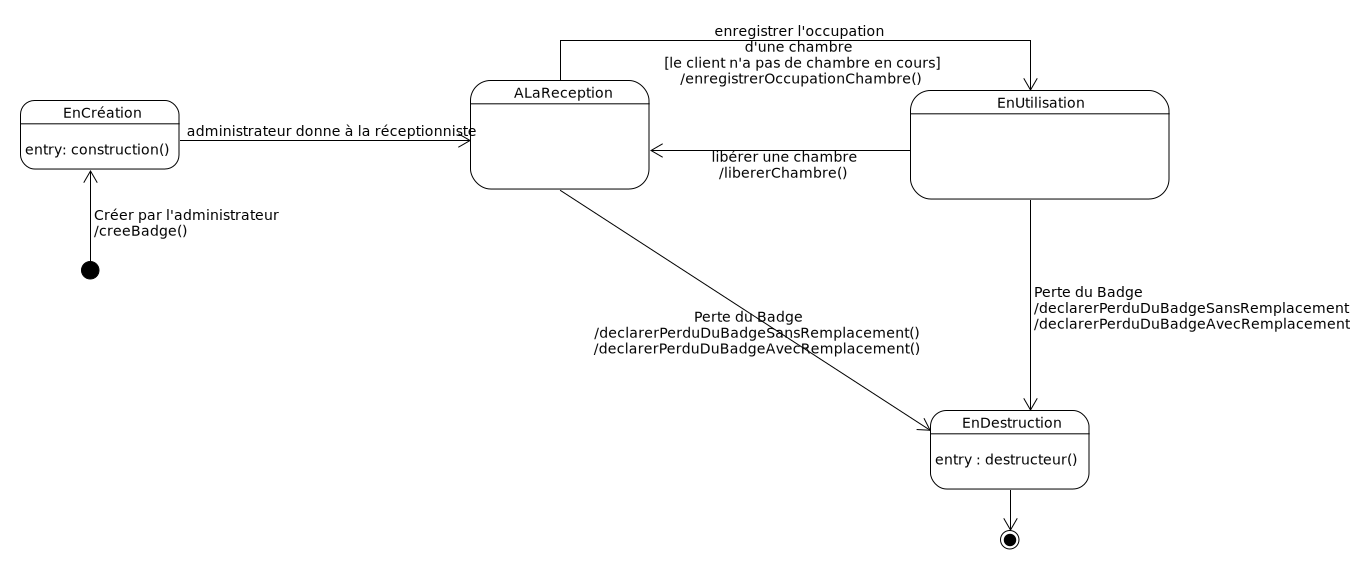
\includegraphics[width=1.3\textwidth,center]{DiagrammesDeMachineAEtats/badge_d_acces}
  \caption{DiagrammesDeMachineAEtats}
  \label{badge_d_acces}

\end{figure}
\bigskip



Invariants :
\bigskip

					( un client associe le badge \\
									\hspace{1cm} $\land$ un chambre associe le badge\\
									\hfill $\land$ les paireClefs de badge $\neq$ null\\
									$\land$ le badge du chambre est pareil que ce badge\\
									$\land$ le badge du client est pareil que ce badge)\\
							$\lor$ \\ (
									$\land$ aucun client associe le badge\\
									$\land$ aucun chambre associe le badge\\
									$\land$ les paireClefs de badge $=$ null\\
							)

\newpage

\section{Préparation des tests unitaires}

    %{\color{red}\textbf{La section est à compléter avec les tables de
    %décision de certaines méthodes des classes les plus importantes.}}

    \begin{table}[htbp!]
        \begin{tabular}{r|p{0.6\linewidth}|c|}
            \cline{2-3}

                &Numéro de test
                &1\\
            \hline
            \hline

            Postcondition
                &badge $\neq$ \nullvalue
                &T\\
            \cline{2-3}
                &paireClefs $=$ \nullvalue
                &T\\
            \cline{2-3}
                &client $=$ \nullvalue
                &T\\
            \cline{2-3}
                &chambre $=$ \nullvalue
                &T\\
            \cline{2-3}
            Exception
                &Levée d'une exception
                &NON\\
            \hline
            \hline
            Effet
                &Création du badge accepté
                &T\\
            \hline
            \hline
                &Nombre de jeux de test
                &1\\
            \cline{2-3}
        \end{tabular}
        \caption{Table de décision du "constructeur" de la classe "Badge"}
    \end{table}

    \begin{table}[htbp!]
        \begin{tabular}{r|p{0.6\linewidth}|c|c|c|c|}
            \cline{2-3}

                &Numéro de test
                &1\\
            \hline
            \hline

            Postcondition
                &client $=$ client
                &T\\
            \cline{2-3}
                &badge.clent $=$ client.badge
                &T\\
            \cline{2-3}
            Exception
                &Levée d'une exception
                &NON\\
            \hline
            \hline
            Effet
                &Association Client Bidirectionnelle accepté pour le badge
                &T\\
            \hline
            \hline
                &Nombre de jeux de test
                &1\\
            \cline{2-3}
        \end{tabular}
        \caption{Table de décision du "AssociationClientBidirectionnelle" de la classe "Badge"}
    \end{table}
\end{document}
